%%
% La siguiente plantilla esta basada en el siguiente enlace:
% http://academic.reed.edu/physics/courses/Physics332.s08/reports.html
% La plantilla original puede descargarse de ese sitio
% Se dejo parte del texto original en inglés para ilustar el uso de la plantilla
% Se hicieron algunas modificaciones para ajustar el idioma y otros detalles para 
% completar un reporte técnico breve pero muy puntual
% Modificación Inicial: Marco Aurelio Nuno Maganda - 11/SEP/2014
% 
% Enlace a la documentación del tipo de documento base (revtex4)
% http://mirror.hmc.edu/ctan/macros/latex/contrib/revtex/doc/latex/revtex/source/revtex4-1.pdf
%
% En algunas distribuciones es necesario instalar el paquete texlive-publishers
%
%\documentclass[letterpaper,aps,twocolumn,pre,nofootinbib]{revtex4}
%\documentclass[twocolumn]{article}
\documentclass[conference]{IEEEtran}

\usepackage[spanish]{babel}
\usepackage{amsmath,amssymb,amsfonts,amsthm}
\usepackage{graphicx}
%\usepackage{bbm}
\usepackage[utf8]{inputenc} % Caracteres en Español (Acentos, ñs)
\usepackage{url} % ACENTOS
\usepackage{hyperref} % Referencias
\usepackage{subfig}
\usepackage{lipsum}
\usepackage{balance}


%%%%%%%%%%%%%%%%%%%%%%%%%%%%%%%%%%%%%%%%%%%%%
% PARCHE PARA ELIMINAR LA FECHA DEL DOCUMENTO
% 
\usepackage{etoolbox}
\makeatletter
% \frontmatter@RRAP@format is responsible for the parentheses
\patchcmd{\frontmatter@RRAP@format}{(}{}{}{}
\patchcmd{\frontmatter@RRAP@format}{)}{}{}{}
%\renewcommand\Dated@name{}
\makeatother	
% FIN DEL PARCHE
% 
%%%%%%%%%%%%%%%%%%%%%%%%%%%%%%%%%%%%%%%%%%%%%

%%%%%%%%%%%%%%%%%%%%%%%%%%%%%%%%%%%%%%%%%%%%%
% PARCHE PARA PERMIRIR UTILIZAR BIBLATEX EN ESTA PANTLLA
%\PassOptionsToPackage{square,numbers}{natbib}
%\RequirePackage{natbib}  
%%%%%%%%%%%%%%%%%%%%%%%%%%%%%%%%%%%%%%%%%%%%%

\usepackage[backend=bibtex,sorting=none]{biblatex}
% Estas lineas permiten romper los hipervinculos muy largos !!!!
\setcounter{biburllcpenalty}{7000}
\setcounter{biburlucpenalty}{8000}
\addbibresource{references.bib}

% Actualiza en automático la fecha de las citas de internet a la fecha de la compilación del documento
\usepackage{datetime}
\newdateformat{specialdate}{\twodigit{\THEDAY}-\twodigit{\THEMONTH}-\THEYEAR}
\date{\specialdate\today}

% la sentencia \burl en las citas... 
\usepackage[hyphenbreaks]{breakurl}

\renewcommand\spanishtablename{Tabla}
\renewcommand\spanishfigurename{Figura}

%\usepackage{datetime}
%\newdateformat{specialdate}{\twodigit{\THEDAY}-\twodigit{\THEMONTH}-\THEYEAR}
%\newdateformat{specialdate}{\twodigit{\THEDAY}-\THEYEAR}
%\date{\specialdate\today}


\begin{document}
%%%%%%%%%%%%%%%%%%%%%%%%%%%%%%%%%%%%%%%%%%%%%
% Definitions
%
%
% Define your special symbols here
%
%%%%%%%%%%%%%%%%%%%%%%%%%%%%%%%%%%%%%%%%%%%%%

% use to set width of figures
\newcommand{\breite}{1.0} %  for twocolumn
\newcommand{\RelacionFiguradoscolumnas}{0.9}
\newcommand{\RelacionFiguradoscolumnasPuntoCinco}{0.45}


%%%%%%%%%%%%%%%%%%%%%%%%%%%%%%%%%%%%%%%%%%%%%
% End Definitions
%%%%%%%%%%%%%%%%%%%%%%%%%%%%%%%%%%%%%%%%%%%%%


%Title of paper
\title{Migración de una Aplicación de Realidad Virtual de la Universidad Politécnica de Victoria de Java a Kotlin para Android}

% Trabajo Individual
%\author{\IEEEauthorblockN{Marco Aurelio Nuno-Maganda\IEEEauthorrefmark{1}}
% En caso de trabajos en equipo, poner a todos los autores en estricto ORDEN ALFABETICO
\author{\IEEEauthorblockN{Nicolas Animas-Arguello \IEEEauthorrefmark{1},
Jesus Emmanuel Lopez-Zuñiga \IEEEauthorrefmark{1},\\
Myriam Elizabeth Pequeño-Aguilera\IEEEauthorrefmark{1}, 
Enrique Ramos-Gallegos\IEEEauthorrefmark{1}}
%Eldon Tyrell\IEEEauthorrefmark{1}}
\IEEEauthorblockA{\IEEEauthorrefmark{1}Ingeniería en Tecnologías de la Información\\
Universidad Politécnica de Victoria}
}


%\date{}

\maketitle

\begin{abstract} 
Este trabajo presenta la migración de una aplicación de realidad virtual para Android, desarrollada originalmente en Java, hacia Kotlin. La aplicación permite recorrer virtualmente las instalaciones de la Universidad Politécnica de Victoria mediante un entorno inmersivo y un control de realidad virtual. Durante la migración se convirtieron las clases del proyecto, se adaptó la configuración necesaria y se verificó el correcto funcionamiento de la aplicación. Como resultado, se obtuvo un proyecto funcional en Kotlin con una estructura de código más moderna y fácil de mantener.
\end{abstract}


%\maketitle must follow title, authors, abstract, \pacs, and \keywords




\section{Introducción}

La realidad virtual (RV) ha experimentado un crecimiento significativo en la última década, impulsada por el desarrollo de dispositivos de visualización, sensores de movimiento y plataformas de desarrollo que permiten crear entornos tridimensionales inmersivos a un costo cada vez más accesible. Esta tecnología facilita a los usuarios la sensación de presencia dentro de un entorno digital mediante la interacción directa con objetos y escenarios, superando las limitaciones de las interfaces tradicionales. Gracias a estas capacidades, la RV se ha integrado exitosamente en ámbitos diversos, tales como la educación, la medicina, la arquitectura, la ingeniería, la capacitación industrial y el entretenimiento \cite{radianti2020, merchant2014}.\\

En el ámbito educativo, la RV se ha consolidado como una herramienta potente para mejorar el proceso de enseñanza-aprendizaje, permitiendo simular entornos o situaciones de difícil acceso en un aula convencional. Investigaciones han demostrado que estos entornos incrementan la motivación del estudiante y fomentan el aprendizaje activo, mejorando notablemente la comprensión espacial en actividades de exploración técnica \cite{radianti2020, freina2015}. Además, la implementación de recorridos virtuales ofrece una solución estratégica para que estudiantes de nuevo ingreso y visitantes conozcan la infraestructura universitaria de forma remota, superando barreras geográficas.\\

Este desarrollo tecnológico ha sido respaldado por la evolución del sistema operativo Android, el cual se mantiene como la plataforma móvil con mayor adopción a nivel global. Android proporciona un robusto ecosistema de herramientas, bibliotecas y APIs que permiten implementar aplicaciones con capacidades gráficas avanzadas y soporte nativo para tecnologías de RV. Por ello, gran parte de las soluciones inmersivas actuales utilizan motores gráficos especializados sobre esta plataforma para el procesamiento de entornos tridimensionales y la gestión de eventos de interacción \cite{androiddevelopers, arcore}.\\

Durante años, Java fue el lenguaje predominante para el desarrollo en Android debido a su madurez y estabilidad. No obstante, ante el aumento en la complejidad de las aplicaciones, surgieron desafíos técnicos relacionados con el manejo de referencias nulas (NullPointerExceptions), la verbosidad del código y los costos de mantenimiento a largo plazo. Estas limitaciones motivaron la transición hacia alternativas más modernas.\\

Como respuesta, surgió Kotlin, un lenguaje desarrollado por JetBrains que se ejecuta sobre la Máquina Virtual de Java (JVM), garantizando interoperabilidad total con el código existente. En 2017, Google otorgó a Kotlin soporte oficial como lenguaje de primera clase para Android, recomendándolo posteriormente como el estándar para el desarrollo de nuevas aplicaciones \cite{kotlinandroid, jetbrains}. Kotlin destaca por características avanzadas como la seguridad contra referencias nulas (Null Safety), inferencia de tipos, corrutinas para programación asíncrona y una sintaxis concisa que reduce drásticamente el código repetitivo (boilerplate), optimizando así la legibilidad y la productividad del desarrollador \cite{kotlindocs}. Asimismo, la compatibilidad total con Java permite realizar migraciones incrementales, reduciendo riesgos en la modernización del software.\\

La literatura científica respalda esta transición: Hecht et al. \cite{hecht2019} analizaron la adopción de Kotlin en proyectos de código abierto, reportando una tendencia creciente tras su oficialización. Por otro lado, Pinto et al. \cite{pinto2021} concluyen que Kotlin mejora directamente la mantenibilidad y reduce la incidencia de errores comunes presentes en implementaciones originales en Java, lo cual valida la migración como una estrategia eficaz de mejora de calidad.\\

En este contexto, el presente trabajo aborda la migración de una aplicación de realidad virtual, desarrollada originalmente para la Universidad Politécnica de Victoria, hacia el lenguaje Kotlin. La aplicación permite realizar un recorrido interactivo por el campus mediante el uso de visores de RV. El proyecto constituye un caso de estudio idóneo para ejecutar un proceso de migración que comprende la conversión de clases, la adaptación de la configuración del proyecto y la validación de la estabilidad del sistema tras el cambio de paradigma.\\

El objetivo central es realizar esta transición preservando la funcionalidad original y aprovechando las ventajas de Kotlin en términos de seguridad, robustez y mantenibilidad, asegurando que la experiencia del usuario final en el recorrido virtual se mantenga intacta tras la actualización tecnológica.\\

\section{Desarrollo Experimental}

El proceso consistió en la migración completa de una aplicación Android implementada originalmente en Java hacia Kotlin, procurando conservar la funcionalidad, la organización del proyecto y la arquitectura definida en la versión original. Debido a que la aplicación representa un sistema con múltiples componentes interdependientes, la migración se realizó de forma incremental, analizando previamente la estructura del proyecto y estableciendo una metodología que permitiera reducir errores de compilación y facilitar la identificación de incompatibilidades entre ambos lenguajes.\\

Antes de iniciar la conversión fue necesario estudiar la organización interna de la aplicación con el propósito de identificar las relaciones entre actividades, clases auxiliares, componentes gráficos y recursos del proyecto. A partir de este análisis se definió una estrategia de migración orientada a preservar la estructura del software y garantizar que cada modificación pudiera validarse antes de continuar con el siguiente componente.\\

\subsection{Análisis de la aplicación original}

Como etapa inicial se realizó un análisis de la estructura del proyecto con el objetivo de identificar los componentes que conforman la aplicación y determinar las dependencias existentes entre ellos. Este análisis permitió conocer la organización de los paquetes, la distribución de las clases y la interacción entre las actividades principales, los modelos de datos, las utilerías y los componentes encargados del renderizado gráfico.\\

La identificación de esta arquitectura permitió establecer una estrategia de migración que respetara la organización original del proyecto, conservando la estructura de paquetes, la nomenclatura de las clases y las dependencias existentes entre los diferentes módulos.

Asimismo, se verificó que el proyecto compilara correctamente en su versión desarrollada en Java, estableciendo una línea base de funcionamiento que posteriormente serviría como referencia para validar la versión migrada.

\subsection{Arquitectura de la aplicación}

La Figura \ref{fig1} presenta la arquitectura general de la aplicación original, organizada en cuatro componentes principales: la capa de presentación, la lógica de la aplicación, el motor de renderizado y los recursos del proyecto. Las actividades (\textit{Activities}) constituyen el punto de interacción con el usuario y son responsables de gestionar los eventos y coordinar la ejecución de la lógica del sistema. Esta última procesa la información, administra los modelos de datos y controla el flujo de ejecución de la aplicación.\\

Por su parte, el motor de renderizado implementa las operaciones necesarias para la representación de los objetos tridimensionales mediante OpenGL ES, haciendo uso de modelos, texturas y demás recursos gráficos almacenados en el proyecto. Finalmente, los recursos de Android, como archivos XML, imágenes y configuraciones, son compartidos entre los distintos componentes para proporcionar tanto la interfaz gráfica como los elementos necesarios para el funcionamiento del sistema.\\

\begin{figure}[!h]
	\includegraphics*[width=\breite \columnwidth]{img1} 
	\caption{Diagrama de componentes que muestra la organización funcional de la aplicación antes del proceso de migración a Kotlin.}
	\label{fig1}
\end{figure}

\subsection{Planeación de la migración}

Una vez comprendida la arquitectura del proyecto se definió una estrategia de migración incremental. El objetivo principal consistió en sustituir gradualmente los archivos implementados en Java por sus equivalentes en Kotlin sin alterar la estructura del proyecto ni modificar el comportamiento observable de la aplicación.\\

Como criterio de trabajo se decidió conservar la organización original de paquetes, la nomenclatura de las clases, la distribución de recursos y el número de archivos existentes en el proyecto. De esta manera fue posible mantener la compatibilidad entre los distintos componentes y facilitar la comparación entre ambas versiones durante el proceso de validación.\\

\subsection{Metodología de la migración}

Con base en el análisis de la arquitectura del proyecto, se definió una metodología de migración incremental orientada a minimizar la introducción de errores y facilitar la validación de cada cambio realizado. La estrategia consistió en migrar un único archivo a la vez, verificando su correcta integración con el resto del sistema antes de continuar con el siguiente componente. La Figura \ref{fig2} resume el flujo de trabajo seguido durante el proceso de migración.\\

\begin{figure}[!h]
	\includegraphics*[width=\breite \columnwidth]{img2} 
	\caption{Flujo de trabajo seguido durante el proceso de migración, compilación y validación de cada archivo del proyecto.}
	\label{fig2}
\end{figure}

\subsection{Modificaciones realizadas}

Al finalizar la migración, se identificó y dio solución a dos fallos principales: 

\subsubsection{Corrección de movimiento opuesto en los controles}

\begin{itemize}
	
	\item \textbf{\textit{Fallo detectado:}} En la versión Java, algunos vectores de desplazamiento y rotación respondían de manera invertida debido a incongruencias en la inversión de signos dentro de la lógica matemática de navegación.\\
	
	\item \textbf{\textit{Solución Aplicada:}} En la nueva versión en Kotlin, se ajustaron los factores de multiplicación vectorial, eliminando los operadores negativos innecesarios, lo que permitió que las direcciones del control correspondieran de manera natural e intuitiva con el desplazamiento del usuario.\\
	
\end{itemize}

\subsubsection{Corrección de desplazamiento diagonal no deseado al avanzar o retroceder}

\begin{itemize}
	
	\vspace{0.5cm}
	
	\item \textbf{\textit{Fallo detectado:}} Al desplazarse hacia adelante o hacia atrás, el sistema en Java utilizaba el vector de dirección completo. Dado que este vector se recalcula directamente a partir de la matriz de rotación del dispositivo para incluir la inclinación vertical (mirar hacia arriba o hacia abajo), el usuario experimentaba una alteración involuntaria de la altura, generando un movimiento diagonal no deseado (flotando o hundiéndose ligeramente).\\
	
	\item \textbf{\textit{Solución Aplicada:}}  En la nueva versión en Kotlin, se modificó la función \textit{MoveForward} aislando únicamente la componente horizontal del vector de dirección. Al ignorar el eje $Y$ para este cálculo específico, se logró que el movimiento de avance y retroceso se mantuviera estrictamente plano sobre el suelo, preservando el vector completo exclusivamente para la renderización de la cámara. \\
	
\end{itemize}

\section{Resultados}

Una vez concluido el proceso de migración se obtuvo una versión funcional de la aplicación desarrollada completamente en Kotlin, manteniendo la arquitectura, la organización del proyecto y el comportamiento general de la versión implementada originalmente en Java. Los resultados obtenidos permiten evaluar el grado de éxito alcanzado durante la conversión y verificar el cumplimiento de los objetivos planteados.\\

\subsection{Resultado de la migración}

\begin{table}[h]
	\centering
	\caption{Resumen del proceso de migración de la aplicación.}
	\label{tab1}
	\begin{tabular}{l|c}
		\textbf{Métrica} & \textbf{Resultado} \\
		\hline
		Lenguaje original & Java \\
		Lenguaje final & Kotlin \\
		Archivos Java originales & 61 \\
		Archivos Kotlin generados & 69 \\
		Estructura de paquetes & Conservada \\
		Nomenclatura de clases & Conservada \\
		Recursos del proyecto & Sin modificaciones \\
		Arquitectura de la aplicación & Conservada \\
		Método de migración & Manual e incremental \\
	\end{tabular}
\end{table}

La Tabla \ref{tab1} resume los principales resultados obtenidos durante la migración. Se observa que el número de archivos se mantuvo constante, lo que permitió conservar la organización original del proyecto y facilitar la comparación entre ambas versiones de la aplicación.\\

\subsection{Conservación de la arquitectura}

Uno de los principales objetivos de la migración consistió en preservar la arquitectura de la aplicación. Para ello se mantuvo la estructura de paquetes, la organización de las clases y las relaciones de dependencia entre los distintos componentes del sistema. Asimismo, los recursos gráficos, archivos de configuración y demás elementos del proyecto permanecieron sin modificaciones, limitando los cambios únicamente al lenguaje de programación utilizado en la implementación.\\

La conservación de esta estructura permitió reducir el impacto de la migración sobre el funcionamiento general de la aplicación y simplificó la validación de los componentes migrados.\\

\subsection{Verificación funcional}

Con el propósito de validar la correcta operación de la aplicación después del proceso de migración, se realizaron pruebas de ejecución sobre los principales escenarios de uso. Estas pruebas consistieron en verificar la carga de los modelos tridimensionales, la navegación dentro del entorno virtual y el acceso al interior de los edificios disponibles en la aplicación. La Figura \ref{fig:edificios} presenta algunas de las capturas obtenidas durante estas pruebas funcionales.\\ \\

\begin{figure}[h]
\centering

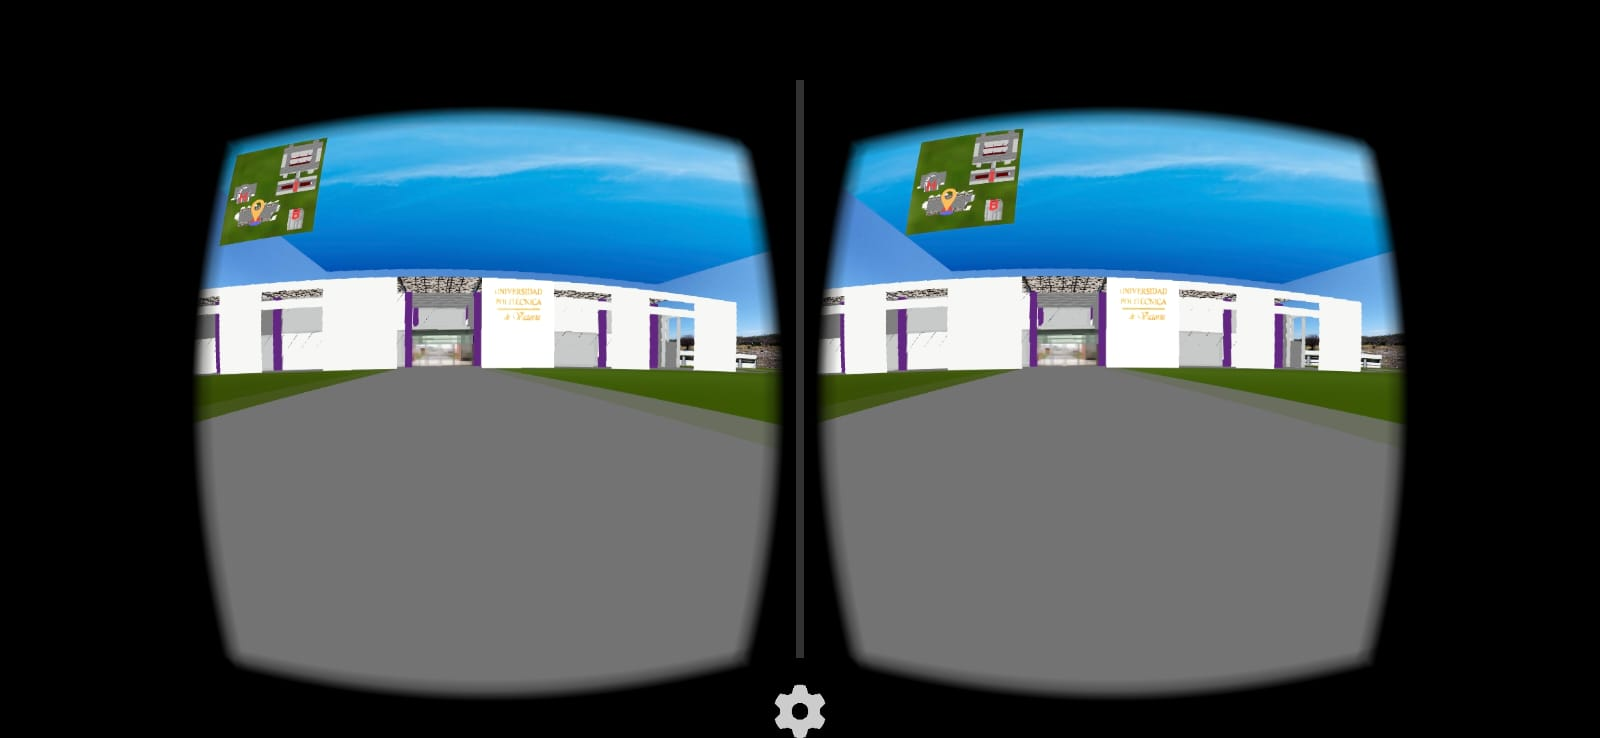
\includegraphics[width=0.42\textwidth]{img3}
\hfill
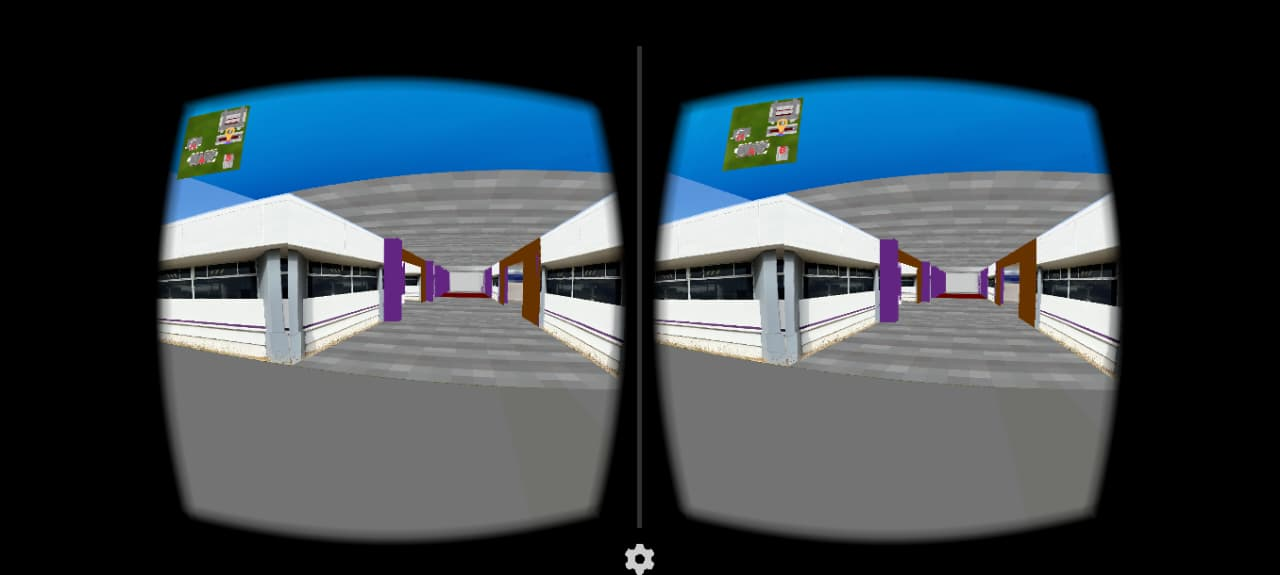
\includegraphics[width=0.42\textwidth]{i}

\vspace{0.4cm}

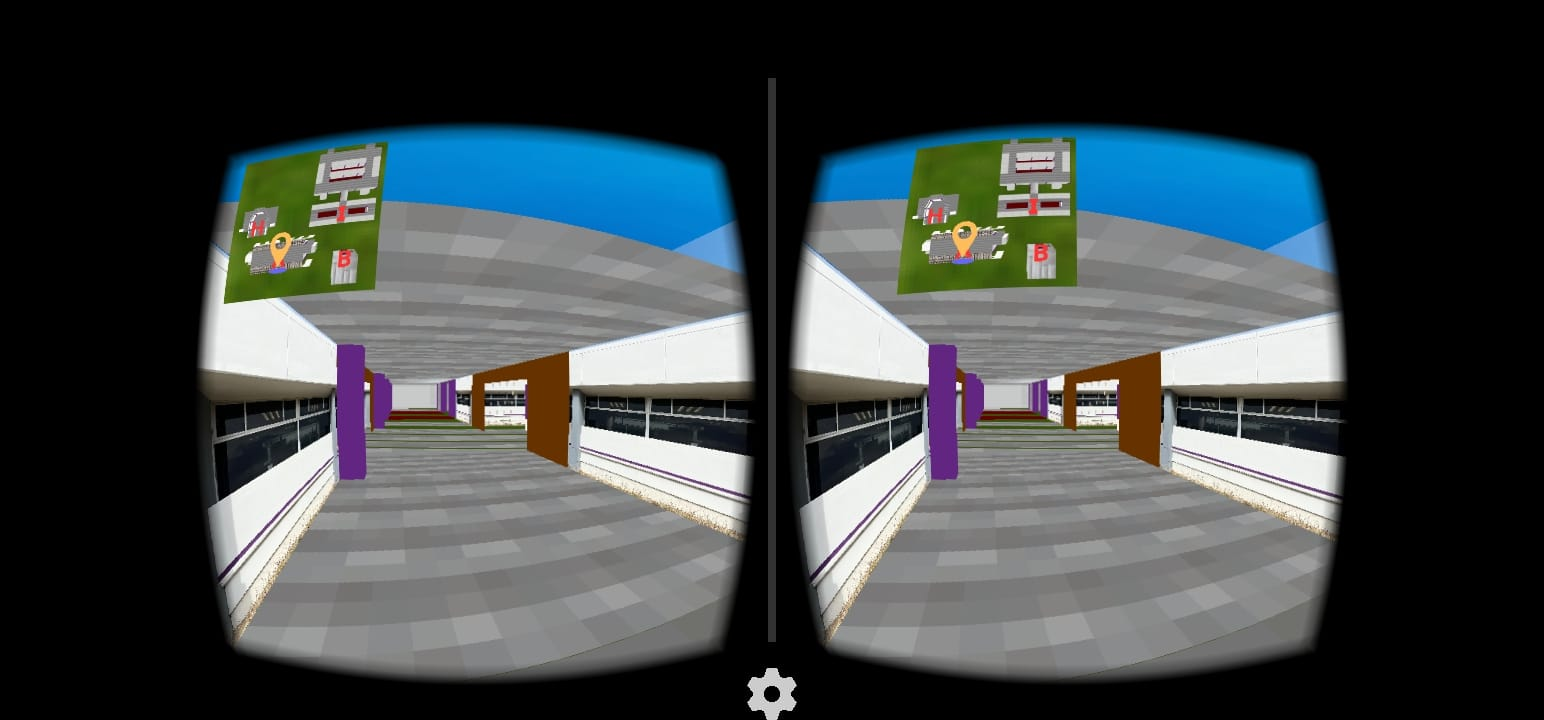
\includegraphics[width=0.42\textwidth]{ia}
\hfill
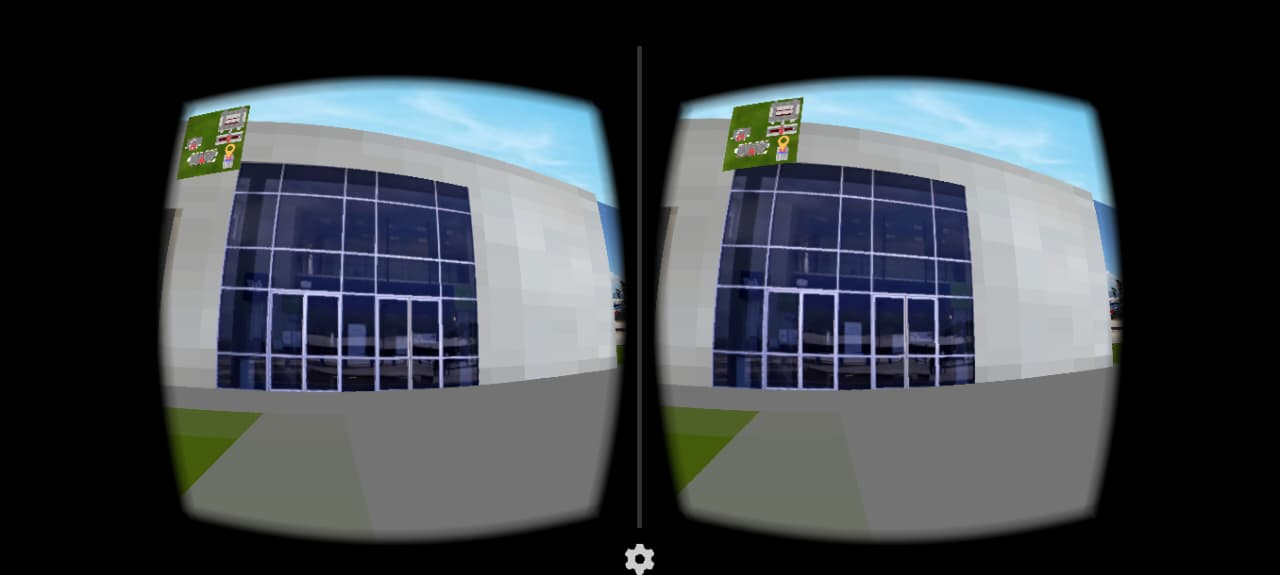
\includegraphics[width=0.42\textwidth]{b}

\vspace{0.4cm}

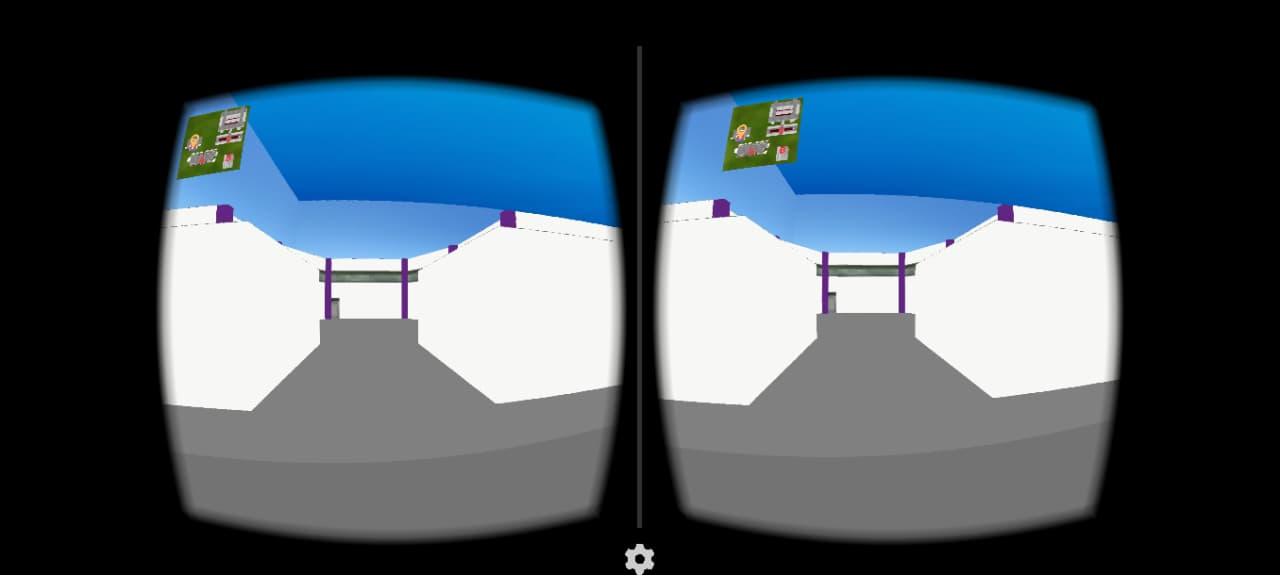
\includegraphics[width=0.42\textwidth]{h}

\caption{Capturas obtenidas durante la ejecución de la aplicación migrada a Kotlin. Se observa la visualización de los edificios A, I, B y H, así como una vista del interior del edificio I, evidenciando el correcto funcionamiento del motor de renderizado y la carga de los recursos gráficos.}
\label{fig:edificios}
\end{figure}

Las capturas muestran que la aplicación conserva la capacidad de representar correctamente los modelos tridimensionales y de cargar los recursos gráficos asociados a cada edificio. Asimismo, la visualización del interior del edificio I confirma que la navegación dentro del entorno virtual continúa funcionando de manera adecuada, lo que indica que la migración de Java a Kotlin no afectó la operación del motor de renderizado ni la interacción con la escena tridimensional.\\ \\

Además, con la finalidad de probar si los errores de la aplicación original en Java fueron realmente solucionados en la nueva versión Kotlin, se realizaron pruebas relacionadas con el control de movimiento y la navegación del usuario en el entorno. \\

La evidencia en video puede ser observada en el siguiente repositorio:\\

\url{https://github.com/EmmanuelLopez15/video_movimiento_upv} 

\section{Conclusión}

La migración de la aplicación de realidad virtual de la Universidad Politécnica de Victoria desde Java hacia Kotlin permitió modernizar la base de código sin afectar las funcionalidades principales del sistema. Durante el proceso fue posible convertir las clases existentes, adaptar la configuración del proyecto y resolver los problemas de compatibilidad propios de la interoperabilidad entre ambos lenguajes, verificando posteriormente el correcto funcionamiento de la aplicación.\\

Los resultados obtenidos demuestran que Kotlin representa una alternativa adecuada para la evolución de aplicaciones Android desarrolladas originalmente en Java, ya que ofrece una sintaxis más concisa, un mejor manejo de referencias nulas y herramientas que facilitan el mantenimiento y la escalabilidad del software. Asimismo, la compatibilidad entre ambos lenguajes permitió realizar una migración gradual, reduciendo el riesgo de introducir errores y evitando la necesidad de reescribir completamente el proyecto.\\

Como resultado de este trabajo se obtuvo una aplicación funcional que conserva la experiencia de recorrido virtual por las instalaciones de la Universidad Politécnica de Victoria, permitiendo al usuario explorar el entorno mediante un control de realidad virtual tal como en la versión original. Además, el proyecto quedó preparado para incorporar futuras mejoras, actualizar dependencias y aprovechar nuevas características del ecosistema Android.\\

Como trabajo futuro, se plantea optimizar el rendimiento de la app e incorporar nuevas funcionalidades que mejoren la interacción del usuario, como sistemas de información contextual, recorridos guiados y una interfaz más intuitiva, fortaleciendo así la experiencia ofrecida por la aplicación.\\

\addcontentsline{toc}{section}{Referencias} 
\printbibliography
%\balance



\end{document}













